\documentclass[aspectratio=169,12pt]{beamer}

% =====================================================================
% THEME AND COLORS
% =====================================================================
\usetheme{Madrid}
\usecolortheme{default}

% Harvard crimson palette
\definecolor{harvardcrimson}{RGB}{165,28,48}
\definecolor{harvardblack}{RGB}{30,30,30}
\definecolor{harvardgray}{RGB}{120,120,120}
\definecolor{lightgray}{RGB}{240,240,240}
\definecolor{accentblue}{RGB}{41,89,149}

\setbeamercolor{structure}{fg=harvardcrimson}
\setbeamercolor{title}{fg=white,bg=harvardcrimson}
\setbeamercolor{frametitle}{fg=harvardcrimson,bg=white}
\setbeamercolor{block title}{fg=white,bg=harvardcrimson}
\setbeamercolor{block body}{bg=lightgray}
\setbeamercolor{item}{fg=harvardcrimson}
\setbeamercolor{footline}{fg=harvardgray}

\setbeamerfont{title}{size=\Large,series=\bfseries}
\setbeamerfont{frametitle}{size=\large,series=\bfseries}
\setbeamerfont{footnote}{size=\tiny}

% Remove navigation symbols
\setbeamertemplate{navigation symbols}{}

% Slide numbers
\setbeamertemplate{footline}{%
  \hfill\insertframenumber/\inserttotalframenumber\hspace{2em}\vspace{1em}%
}

% =====================================================================
% PACKAGES
% =====================================================================
\usepackage{graphicx}
\usepackage{booktabs}
\usepackage{tikz}
\usetikzlibrary{shapes.geometric, arrows.meta, positioning, calc}
\usepackage{xcolor}
% If using XeLaTeX, uncomment the next two lines:
% \usepackage{fontspec}
% \setmainfont{Times New Roman}
% If using pdfLaTeX, use this instead:
\usepackage{mathptmx} % Times Roman font for pdfLaTeX

% =====================================================================
% TITLE
% =====================================================================
\title[Board Observers]{The Three-Tier Board:\\Directors, Observers, and Advisors\\in Venture-Backed Governance}
\author{Harp Jung}
\institute{Harvard University}
\date{March 2026}

\begin{document}

% =====================================================================
% TITLE SLIDE
% =====================================================================
\begin{frame}
\titlepage
\end{frame}

% =====================================================================
% BEAT 1: THE INTERVIEW JOURNEY
% =====================================================================
\section{The Interview Journey}

\begin{frame}{Research Starting Point}
\begin{center}
\Large\textbf{What makes a board effective?}
\end{center}
\vspace{1em}
\begin{itemize}
\item Who sits on the board, what roles do they play, and how does that shape governance?
\item Rich literature on director independence, composition, and monitoring --- but almost entirely focused on formal directors
\item \textbf{My approach:} Talk to practitioners who actually sit on these boards
\end{itemize}
\end{frame}

\begin{frame}{Three Practitioner Interviews}
\begin{center}
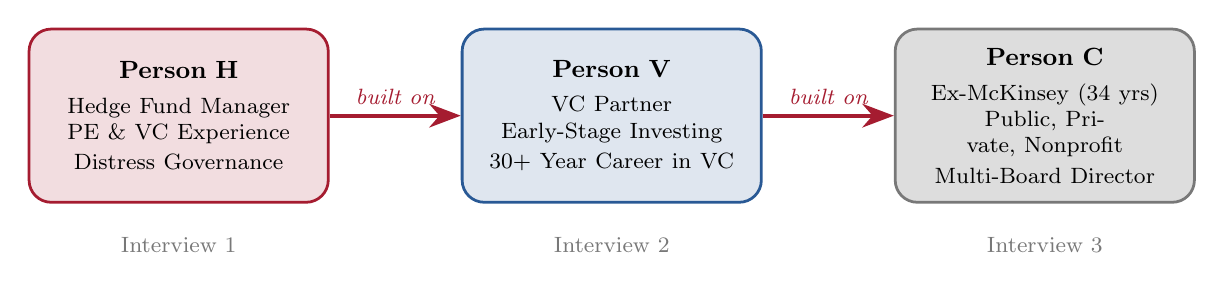
\begin{tikzpicture}[
    box/.style={rounded corners=8pt, minimum width=3.8cm, minimum height=2.2cm, text width=3.4cm, align=center, font=\small},
    arrow/.style={-{Stealth[length=4mm]}, line width=1.5pt, harvardcrimson}
]
% Three boxes
\node[box, fill=harvardcrimson!15, draw=harvardcrimson, line width=1pt] (H) at (0,0) {
    \textbf{Person H}\\[3pt]
    \footnotesize Hedge Fund Manager\\
    \footnotesize PE \& VC Experience\\
    \footnotesize Distress Governance
};
\node[box, fill=accentblue!15, draw=accentblue, line width=1pt] (V) at (5.5,0) {
    \textbf{Person V}\\[3pt]
    \footnotesize VC Partner\\
    \footnotesize Early-Stage Investing\\
    \footnotesize 30+ Year Career in VC
};
\node[box, fill=harvardgray!25, draw=harvardgray, line width=1pt] (C) at (11,0) {
    \textbf{Person C}\\[3pt]
    \footnotesize Ex-McKinsey (34 yrs)\\
    \footnotesize Public, Private, Nonprofit\\
    \footnotesize Multi-Board Director
};

% Arrows
\draw[arrow] (H) -- (V) node[midway, above, font=\footnotesize\itshape] {built on};
\draw[arrow] (V) -- (C) node[midway, above, font=\footnotesize\itshape] {built on};

% Labels below
\node[below=0.3cm of H, font=\footnotesize\color{harvardgray}] {Interview 1};
\node[below=0.3cm of V, font=\footnotesize\color{harvardgray}] {Interview 2};
\node[below=0.3cm of C, font=\footnotesize\color{harvardgray}] {Interview 3};

\end{tikzpicture}
\end{center}
\vspace{0.5em}
\begin{center}
\small\textit{Each interview built on the discoveries of the previous one.\\I entered expecting to study the Board of Directors...}
\end{center}
\end{frame}

% =====================================================================
% BEAT 2: THE DISCOVERY MOMENT (PERSON H)
% =====================================================================
\section{The Discovery: Person H}

\begin{frame}{Interview 1: An Unexpected Finding}
\begin{block}{Person H --- Hedge Fund Manager with VC/PE Experience}
\begin{itemize}
\item Has extensive startup board experience
\item But \textbf{NOT} as a board director
\item Served as a \textbf{board observer} and \textbf{board advisor}
\item ``Knows what's going on'' --- could answer anything about governance
\end{itemize}
\end{block}
\vspace{0.5em}
\begin{alertblock}{The Discovery}
I had never heard of a ``board observer'' before this interview.\\
I had heard of advisory board members --- but \textit{observers}?
\end{alertblock}
\end{frame}

\begin{frame}{What Are These Three Roles?}
\small
\begin{block}{Definitions from the Literature}
\begin{description}
\item[\textcolor{harvardcrimson}{Directors}] Formally elected, voting members with fiduciary duties of care and loyalty. Average startup board: 4.5 directors (2 VCs, 1.7 executives, 0.8 independent). \\ \hfill\textit{\footnotesize --- Ewens \& Malenko (2024)}
\vspace{0.3em}
\item[\textcolor{accentblue}{Observers}] ``Individuals without voting rights who serve as strategic eyes on the board, providing insight and influence without the fiduciary responsibilities of board membership.'' \\ \hfill\textit{\footnotesize --- Packin \& Alon-Beck (2025, p.\ 1508)}
\vspace{0.3em}
\item[\textcolor{harvardgray}{Advisors}] Honorary roles providing domain expertise and network access. ``The firm could establish an advisory board (as is frequently done in private firms).'' \\ \hfill\textit{\footnotesize --- Ewens \& Malenko (2024, fn.\ 3)}
\end{description}
\end{block}
\end{frame}

\begin{frame}{The Three Tiers: A Comparison}
\centering
\footnotesize
\begin{tabular}{@{}l c c c@{}}
\toprule
\textbf{Attribute} & \textbf{Directors (Tier 1)} & \textbf{Observers (Tier 2)} & \textbf{Advisors (Tier 3)} \\
\midrule
Voting Rights & \textcolor{harvardcrimson}{\textbf{Yes}} & No & No \\
Fiduciary Duty & \textcolor{harvardcrimson}{\textbf{Yes}} & \textbf{No} & No \\
Information Access & Full & \textbf{Full (same as directors)} & Limited \\
Personal Liability & Yes (+ D\&O) & \textbf{No} & No \\
Legal Basis & Charter, bylaws & IRA (contractual) & Informal \\
\addlinespace
Prevalence in VC & Universal & \textbf{82\% of VC entities} & Common but informal \\
\bottomrule
\end{tabular}
\vspace{0.5em}

\textit{\scriptsize Sources: Ewens \& Malenko (2024); Packin \& Alon-Beck (2025); NVCA Q4 2023 CFO Survey}
\end{frame}

% =====================================================================
% BEAT 3: LITERATURE DEEP DIVE
% =====================================================================
\section{Prior Literature}

\begin{frame}{Startup Boards Are Different}
\begin{columns}
\begin{column}{0.55\textwidth}
\textbf{Ewens \& Malenko (2024):} \\
7,780 startups, 2002--2017
\begin{itemize}
\item Board control shifts over lifecycle:
\begin{itemize}
    \footnotesize
    \item 1st financing: 47\% entrepreneur-controlled
    \item 2nd financing: 36\% shared control
    \item 4th financing: 62\% VC-controlled
\end{itemize}
\item Independent directors play a \textbf{mediation} role (not just monitoring)
\item Data tracks 3 types: executive, VC, independent
\item \textcolor{harvardcrimson}{\textbf{Observers acknowledged in fn.\ 3 but NOT studied}}
\end{itemize}
\end{column}
\begin{column}{0.42\textwidth}
\centering
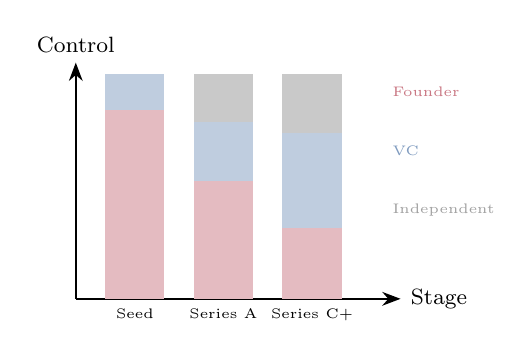
\begin{tikzpicture}[scale=0.75]
% Simple lifecycle diagram
\draw[-{Stealth}, thick] (0,0) -- (5.5,0) node[right]{\footnotesize Stage};
\draw[-{Stealth}, thick] (0,0) -- (0,4) node[above]{\footnotesize Control};

% Bars
\fill[harvardcrimson!30] (0.5,0) rectangle (1.5,3.2);
\fill[accentblue!30] (0.5,3.2) rectangle (1.5,3.8);
\node[below, font=\tiny] at (1,0) {Seed};

\fill[harvardcrimson!30] (2,0) rectangle (3,2.0);
\fill[accentblue!30] (2,2.0) rectangle (3,3.0);
\fill[harvardgray!40] (2,3.0) rectangle (3,3.8);
\node[below, font=\tiny] at (2.5,0) {Series A};

\fill[harvardcrimson!30] (3.5,0) rectangle (4.5,1.2);
\fill[accentblue!30] (3.5,1.2) rectangle (4.5,2.8);
\fill[harvardgray!40] (3.5,2.8) rectangle (4.5,3.8);
\node[below, font=\tiny] at (4,0) {Series C+};

% Legend
\node[font=\tiny, right] at (5.2,3.5) {\textcolor{harvardcrimson!60}{Founder}};
\node[font=\tiny, right] at (5.2,2.5) {\textcolor{accentblue!60}{VC}};
\node[font=\tiny, right] at (5.2,1.5) {\textcolor{harvardgray!70}{Independent}};
\end{tikzpicture}
\end{column}
\end{columns}
\end{frame}

\begin{frame}{How Prevalent Are Board Observers?}
\begin{block}{NVCA Q4 2023 CFO Working-Group Survey \hfill\small\textit{Packin \& Alon-Beck (2025)}}
\centering
\vspace{0.3em}
\footnotesize
\begin{tabular}{@{}l r@{}}
\toprule
\textbf{Statistic} & \textbf{Finding} \\
\midrule
Overall adoption rate & \textbf{82\%} of VC entities (38 of 46) \\
AUM $>$ \$500M & \textbf{100\%} adoption \\
Traditional VCs & \textbf{Unanimous} adoption \\
Portfolio coverage ($>$75\%) & 10 entities \\
Portfolio coverage (25--75\%) & 16 entities \\
Plans to increase observers & 8 entities \\
\bottomrule
\end{tabular}
\end{block}
\vspace{0.5em}
\begin{center}
\large\textbf{Board observers are the norm, not the exception.}
\end{center}
\end{frame}

\begin{frame}{Packin \& Alon-Beck (2025): The Foundational Paper}
\textit{``Board Observers,'' University of Illinois Law Review}
\vspace{0.3em}
\begin{itemize}
\item \textbf{First academic article} to systematically explore board observers
\item Defines observers as \textbf{``control without formal control''}
\item Legal status: \textit{Obasi v.\ Tibet Pharmaceuticals} (3d Cir.\ 2019) --- observers are NOT directors
\begin{itemize}
    \footnotesize
    \item No voting rights
    \item Tenure not dependent on shareholders
    \item No fiduciary duty to shareholders
\end{itemize}
\item Contractual basis: appointed via IRAs, term sheets, side letters
\item ``Fiduciary duties, or the lack thereof, for board observers in the U.S.\ represent a \textbf{critical issue that warrants further research}'' (p.\ 1564)
\end{itemize}
\end{frame}

% =====================================================================
% BEAT 4: INTERVIEW V --- GROUND TRUTH
% =====================================================================
\section{Ground Truth: Person V}

\begin{frame}{Interview 2: Testing the Literature}
\begin{block}{Objective}
Validate what I learned from the literature with Person V --- a VC partner with a 30+ year career in early-stage investing.
\end{block}
\vspace{0.5em}
\textbf{V's Verdict:} The literature gets the \textit{formal} distinctions right, but misses the \textit{practical} reality.

\vspace{0.5em}
\begin{columns}
\begin{column}{0.48\textwidth}
\begin{alertblock}{Advisors: Nonexistent}
\small
``Almost always more of an honorary position where you're sort of lending your name.'' \\[3pt]
``Never meets... I don't even really talk to them that often.''
\end{alertblock}
\end{column}
\begin{column}{0.48\textwidth}
\begin{exampleblock}{Observers: Near-Directors}
\small
``Very much like a board member... there's just not that much difference.'' \\[3pt]
Yet: completely different legal liability.
\end{exampleblock}
\end{column}
\end{columns}
\end{frame}

\begin{frame}{Four Types of Board Observers}
\small
\textit{Taxonomy from Suster (2019), validated by Persons V and H}
\vspace{0.3em}

\begin{enumerate}
\item \textbf{VC ``Plus-1s''} --- Junior partners brought for training \\
\textcolor{harvardgray}{\footnotesize V: ``You get a board seat, and then you say, [name], [fund]'s partner... particularly when things start to start to go south''}

\item \textbf{Strategic Investors} --- CVCs preferring limited exposure \\
\textcolor{harvardgray}{\footnotesize V: Corporate investors ``very much want to be deemed a competitor on any situation where they might have a conflict''}

\item \textbf{Minority Shareholders} --- Late-round, small-check investors \\
\textcolor{harvardgray}{\footnotesize Negotiation compromise: access without a seat}

\item \textbf{VCs Avoiding Obligation} --- Influence without liability \\
\textcolor{harvardcrimson}{\footnotesize H: ``We still want observation... but we don't want the responsibility''}
\end{enumerate}
\end{frame}

\begin{frame}{The Board Degradation Problem}
\begin{columns}
\begin{column}{0.55\textwidth}
\textbf{As observers proliferate, board dynamics transform:}
\vspace{0.5em}

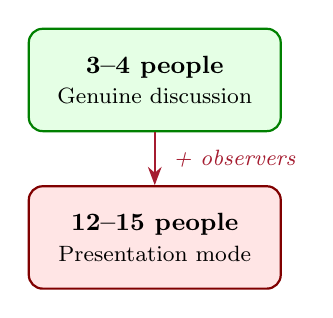
\begin{tikzpicture}[
    box/.style={rounded corners=5pt, minimum width=3.2cm, minimum height=1.3cm, align=center, font=\small, draw, line width=0.8pt}
]
\node[box, fill=green!10, draw=green!50!black] (small) at (0,2) {
    \textbf{3--4 people}\\
    \footnotesize Genuine discussion
};
\node[box, fill=red!10, draw=red!50!black] (large) at (0,0) {
    \textbf{12--15 people}\\
    \footnotesize Presentation mode
};
\draw[-{Stealth}, thick, harvardcrimson] (small) -- (large) node[midway, right, font=\footnotesize\itshape, xshift=3pt] {+ observers};
\end{tikzpicture}
\end{column}
\begin{column}{0.42\textwidth}
\begin{block}{Person V}
\small
``12 or 15 people in the room. That's no longer even, really, much of a discussion. It's more like a presentation.''
\end{block}
\vspace{0.3em}
\begin{block}{Suster (2019)}
\small
``Your five-person board is really an eight-person `board.'\,''
\end{block}
\end{column}
\end{columns}
\vspace{0.5em}
\begin{center}
\small V: ``Almost nothing controversial is EVER voted on... So the value of a person in the room is the value of their speaking.''
\end{center}
\end{frame}

\begin{frame}{The Key Insight from V}
\begin{center}
\Large
\textit{``For all intents and purposes a board observer\\ is like a full board member.''}\\[8pt]
\normalsize --- Suster (2019), confirmed by Person V
\end{center}
\vspace{1em}
\begin{center}
\textbf{Same information. Same meetings. Same influence.}\\[6pt]
\textcolor{harvardcrimson}{\textbf{Zero fiduciary duty. Zero liability. Zero accountability.}}
\end{center}
\end{frame}

% =====================================================================
% BEAT 5: INTERVIEW C --- BOUNDARIES
% =====================================================================
\section{Testing Boundaries: Person C}

\begin{frame}{Interview 3: Is This Just a Startup Thing?}
\begin{block}{Person C --- Ex-McKinsey, Multi-Board Director}
\small
Public board (Leidos), nonprofit (MITRE), family-owned (Huber), financial (Bain Capital BDC). 34 years at McKinsey. HBS faculty.
\end{block}
\vspace{0.5em}
\textbf{Finding:} Board observers are \textbf{not prevalent} outside VC-backed startups.
\begin{itemize}
\item Some PE firms, smaller VCs use them --- but not widespread in public, family, or nonprofit governance
\item C was more familiar with the traditional director model
\end{itemize}

\vspace{0.5em}
\begin{exampleblock}{On Effective Board Membership (Fun Aside)}
\small
\textbf{C and Suster agree:} Read materials beforehand, really get to know the firm --- go visit, interview employees. ``Most of the value comes outside of the boardroom.''
\end{exampleblock}

\vspace{0.3em}
\begin{center}
\textbf{$\Rightarrow$ Board observers are a \textcolor{harvardcrimson}{distinctly VC/startup phenomenon}.}
\end{center}
\end{frame}

% =====================================================================
% BEAT 6: THE ACCOUNTABILITY GAP
% =====================================================================
\section{The Accountability Gap}

\begin{frame}{Five Reasons Observers Escape Accountability}
\small
\textit{Packin \& Alon-Beck (2025) --- Legal Framework}
\vspace{0.3em}

\begin{enumerate}
\item \textbf{No Fiduciary Duty} \\
\footnotesize ``Observers do not owe fiduciary duties to the business entities on the boards of which they serve'' (p.\ 1517)
\normalsize

\item \textbf{Full Information Access} \\
\footnotesize Same materials, same meetings --- but no obligation to act on what they learn

\item \textbf{Antitrust Bypass (Clayton Act \S 8)} \\
\footnotesize ``Board observers are neither officers nor directors, hence investors may use them... without triggering Section 8 liability'' (p.\ 1552)

\item \textbf{CFIUS Workaround} \\
\footnotesize Foreign investors avoid national security review triggers

\item \textbf{Liability Shield (\textit{Obasi} Case)} \\
\footnotesize Courts confirmed: observers $\neq$ directors for liability purposes (3d Cir.\ 2019)
\end{enumerate}
\end{frame}

\begin{frame}{D\&O Insurance Completes the Vacuum}
\begin{columns}
\begin{column}{0.48\textwidth}
\begin{block}{Person H}
\small
``D\&O is almost a prerequisite to being on a board.''\\[6pt]
``Does it make you care less? Maybe... that's actually a hard way to put it, but it kind of... it allows you to care less.''
\end{block}
\end{column}
\begin{column}{0.48\textwidth}
\begin{block}{Person V}
\small
Personal D\&O insurance: \$37,000/year.\\[6pt]
Company D\&O likely does not cover observers: ``I don't think I actually have any liability.''
\end{block}
\end{column}
\end{columns}
\vspace{0.8em}
\begin{center}
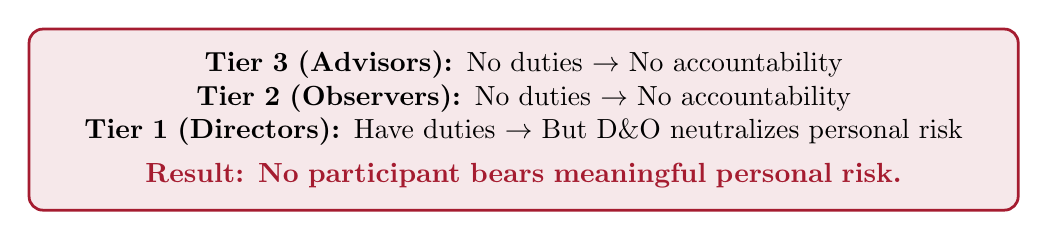
\begin{tikzpicture}
\node[rounded corners=5pt, fill=harvardcrimson!10, draw=harvardcrimson, line width=1pt, text width=12cm, align=center, inner sep=8pt] {
    \textbf{Tier 3 (Advisors):} No duties $\rightarrow$ No accountability \\
    \textbf{Tier 2 (Observers):} No duties $\rightarrow$ No accountability \\
    \textbf{Tier 1 (Directors):} Have duties $\rightarrow$ But D\&O neutralizes personal risk \\[4pt]
    \textcolor{harvardcrimson}{\textbf{Result: No participant bears meaningful personal risk.}}
};
\end{tikzpicture}
\end{center}
\end{frame}

\begin{frame}{The Academic Mandate}
\begin{center}
\large
Carter (\textit{Journal of Accounting \& Economics}, 2025):
\end{center}
\vspace{0.5em}
\begin{block}{}
\centering
\textit{``Board observers may provide a conduit for information, yielding benefits similar to competitor interlocking directors and possibly remain under the DOJ radar.}\\[6pt]
\textit{\textbf{Future research might examine how prevalent they are in public companies and how their presence impacts corporate governance and firm performance.}''}
\end{block}
\vspace{1em}
\begin{center}
\Large\textbf{Not a single business paper has empirically studied board observers.}\\[8pt]
\large\textcolor{harvardcrimson}{So I built the data and tested it.}
\end{center}
\end{frame}

% =====================================================================
% BEAT 7: RESEARCH DESIGN & RESULTS (PLACEHOLDER)
% =====================================================================
\section{Research Design \& Preliminary Results}

\begin{frame}{Data and Sample}
\begin{center}
\Large\textcolor{harvardgray}{\textit{[To be populated after finalizing test specifications]}}
\end{center}
\vspace{1em}
\begin{itemize}
\item S\&P Capital IQ: 3,058 companies with board observer data
\item SEC EDGAR S-1 filings: 320 IRA exhibits coded for observer provisions
\item SEC Form D: 466K private placements, 1.7M related persons
\item CRSP / Compustat / IBES for post-IPO outcomes
\item Observer $\rightarrow$ VC $\rightarrow$ portfolio company network (42,857 positions)
\end{itemize}
\end{frame}

\begin{frame}{Research Questions}
\begin{center}
\Large\textcolor{harvardgray}{\textit{[To be populated]}}
\end{center}
\vspace{1em}
\begin{enumerate}
\item Do observers affect firm governance outcomes?
\item Does information flow through observer networks?
\item Does the accountability structure matter for information flow?
\end{enumerate}
\end{frame}

\begin{frame}{Preliminary Results}
\begin{center}
\Large\textcolor{harvardgray}{\textit{[To be populated after re-running tests]}}
\end{center}
\end{frame}

% =====================================================================
% CLOSING
% =====================================================================
\section{}

\begin{frame}{}
\begin{center}
\vspace{2em}
\Large\textbf{Thank You}\\[1em]
\normalsize
Harp Jung\\
Harvard University\\[1em]
\small\textcolor{harvardgray}{Comments welcome.}
\end{center}
\end{frame}

\end{document}
